%% This is a base file to be used as a template for submitting papers
%% to SET International Journal of Broadcast Engineering - SET IJBE
%% (requires IEEEtran.cls version 1.8b or later).
%%
%% Support: IJBE@set.org.br
%% https://revistas.set.org.br/ijbe
%%
%% Based on IEEE journal template by Michael Shell, available on Overleaf

%%*************************************************************************
%% Legal Notice:
%% This code is offered as-is without any warranty either expressed or
%% implied; without even the implied warranty of MERCHANTABILITY or
%% FITNESS FOR A PARTICULAR PURPOSE! 
%% User assumes all risk.
%% In no event shall the IEEE or any contributor to this code be liable for
%% any damages or losses, including, but not limited to, incidental,
%% consequential, or any other damages, resulting from the use or misuse
%% of any information contained here.
%%
%% All comments are the opinions of their respective authors and are not
%% necessarily endorsed by the IEEE.
%%
%% This work is distributed under the LaTeX Project Public License (LPPL)
%% ( http://www.latex-project.org/ ) version 1.3, and may be freely used,
%% distributed and modified. A copy of the LPPL, version 1.3, is included
%% in the base LaTeX documentation of all distributions of LaTeX released
%% 2003/12/01 or later.
%% Retain all contribution notices and credits.
%%*************************************************************************

\documentclass[journal]{IEEEtran}

% Useful LaTeX packages
\usepackage[spanish]{babel} 
\usepackage[utf8]{inputenc}
\usepackage{cite}
\usepackage{graphicx}
\usepackage{amsmath,amssymb,amsfonts}
\usepackage{algorithmic}
\usepackage{textcomp}
\usepackage{xcolor}
\usepackage{url}
\usepackage{listings}
\usepackage[hidelinks]{hyperref}

% *** MISC UTILITY PACKAGES ***
%
\usepackage{ifpdf}
% Heiko Oberdiek's ifpdf.sty is very useful if you need conditional
% compilation based on whether the output is pdf or dvi.
% usage:
% \ifpdf
%   % pdf code
% \else
%   % dvi code
% \fi
% The latest version of ifpdf.sty can be obtained from:
% http://www.ctan.org/pkg/ifpdf
% Also, note that IEEEtran.cls V1.7 and later provides a builtin
% \ifCLASSINFOpdf conditional that works the same way.
% When switching from latex to pdflatex and vice-versa, the compiler may
% have to be run twice to clear warning/error messages.

% *** CITATION PACKAGES ***
%
%\usepackage{cite}
% cite.sty was written by Donald Arseneau
% V1.6 and later of IEEEtran pre-defines the format of the cite.sty package
% \cite{} output to follow that of the IEEE. Loading the cite package will
% result in citation numbers being automatically sorted and properly
% "compressed/ranged". e.g., [1], [9], [2], [7], [5], [6] without using
% cite.sty will become [1], [2], [5]--[7], [9] using cite.sty. cite.sty's
% \cite will automatically add leading space, if needed. Use cite.sty's
% noadjust option (cite.sty V3.8 and later) if you want to turn this off
% such as if a citation ever needs to be enclosed in parenthesis.
% cite.sty is already installed on most LaTeX systems. Be sure and use
% version 5.0 (2009-03-20) and later if using hyperref.sty.
% The latest version can be obtained at:
% http://www.ctan.org/pkg/cite
% The documentation is contained in the cite.sty file itself.

% *** GRAPHICS RELATED PACKAGES ***
%
\ifCLASSINFOpdf
  % \usepackage[pdftex]{graphicx}
  % declare the path(s) where your graphic files are
  % \graphicspath{{../pdf/}{../jpeg/}}
  % and their extensions so you won't have to specify these with
  % every instance of \includegraphics
  % \DeclareGraphicsExtensions{.pdf,.jpeg,.png}
\else
  % or other class option (dvipsone, dvipdf, if not using dvips). graphicx
  % will default to the driver specified in the system graphics.cfg if no
  % driver is specified.
  % \usepackage[dvips]{graphicx}
  % declare the path(s) where your graphic files are
  % \graphicspath{{../eps/}}
  % and their extensions so you won't have to specify these with
  % every instance of \includegraphics
  % \DeclareGraphicsExtensions{.eps}
\fi
% graphicx was written by David Carlisle and Sebastian Rahtz. It is
% required if you want graphics, photos, etc. graphicx.sty is already
% installed on most LaTeX systems. The latest version and documentation
% can be obtained at: 
% http://www.ctan.org/pkg/graphicx
% Another good source of documentation is "Using Imported Graphics in
% LaTeX2e" by Keith Reckdahl which can be found at:
% http://www.ctan.org/pkg/epslatex
%
% latex, and pdflatex in dvi mode, support graphics in encapsulated
% postscript (.eps) format. pdflatex in pdf mode supports graphics
% in .pdf, .jpeg, .png and .mps (metapost) formats. Users should ensure
% that all non-photo figures use a vector format (.eps, .pdf, .mps) and
% not a bitmapped formats (.jpeg, .png). The IEEE frowns on bitmapped formats
% which can result in "jaggedy"/blurry rendering of lines and letters as
% well as large increases in file sizes.
%
% You can find documentation about the pdfTeX application at:
% http://www.tug.org/applications/pdftex

% *** MATH PACKAGES ***
%
%\usepackage{amsmath}
% A popular package from the American Mathematical Society that provides
% many useful and powerful commands for dealing with mathematics.
%
% Note that the amsmath package sets \interdisplaylinepenalty to 10000
% thus preventing page breaks from occurring within multiline equations. Use:
%\interdisplaylinepenalty=2500
% after loading amsmath to restore such page breaks as IEEEtran.cls normally
% does. amsmath.sty is already installed on most LaTeX systems. The latest
% version and documentation can be obtained at:
% http://www.ctan.org/pkg/amsmath

% *** SPECIALIZED LIST PACKAGES ***
%
%\usepackage{algorithmic}
% algorithmic.sty was written by Peter Williams and Rogerio Brito.
% This package provides an algorithmic environment fo describing algorithms.
% You can use the algorithmic environment in-text or within a figure
% environment to provide for a floating algorithm. Do NOT use the algorithm
% floating environment provided by algorithm.sty (by the same authors) or
% algorithm2e.sty (by Christophe Fiorio) as the IEEE does not use dedicated
% algorithm float types and packages that provide these will not provide
% correct IEEE style captions. The latest version and documentation of
% algorithmic.sty can be obtained at:
% http://www.ctan.org/pkg/algorithms
% Also of interest may be the (relatively newer and more customizable)
% algorithmicx.sty package by Szasz Janos:
% http://www.ctan.org/pkg/algorithmicx


% *** ALIGNMENT PACKAGES ***
%
%\usepackage{array}
% Frank Mittelbach's and David Carlisle's array.sty patches and improves
% the standard LaTeX2e array and tabular environments to provide better
% appearance and additional user controls. As the default LaTeX2e table
% generation code is lacking to the point of almost being broken with
% respect to the quality of the end results, all users are strongly
% advised to use an enhanced (at the very least that provided by array.sty)
% set of table tools. array.sty is already installed on most systems. The
% latest version and documentation can be obtained at:
% http://www.ctan.org/pkg/array


% IEEEtran contains the IEEEeqnarray family of commands that can be used to
% generate multiline equations as well as matrices, tables, etc., of high
% quality.

% *** SUBFIGURE PACKAGES ***
%\ifCLASSOPTIONcompsoc
%  \usepackage[caption=false,font=normalsize,labelfont=sf,textfont=sf]{subfig}
%\else
%  \usepackage[caption=false,font=footnotesize]{subfig}
%\fi
% subfig.sty, written by Steven Douglas Cochran, is the modern replacement
% for subfigure.sty, the latter of which is no longer maintained and is
% incompatible with some LaTeX packages including fixltx2e. However,
% subfig.sty requires and automatically loads Axel Sommerfeldt's caption.sty
% which will override IEEEtran.cls' handling of captions and this will result
% in non-IEEE style figure/table captions. To prevent this problem, be sure
% and invoke subfig.sty's "caption=false" package option (available since
% subfig.sty version 1.3, 2005/06/28) as this is will preserve IEEEtran.cls
% handling of captions.
% Note that the Computer Society format requires a larger sans serif font
% than the serif footnote size font used in traditional IEEE formatting
% and thus the need to invoke different subfig.sty package options depending
% on whether compsoc mode has been enabled.
%
% The latest version and documentation of subfig.sty can be obtained at:
% http://www.ctan.org/pkg/subfig



% *** FLOAT PACKAGES ***
%
%\usepackage{fixltx2e}
% fixltx2e, the successor to the earlier fix2col.sty, was written by
% Frank Mittelbach and David Carlisle. This package corrects a few problems
% in the LaTeX2e kernel, the most notable of which is that in current
% LaTeX2e releases, the ordering of single and double column floats is not
% guaranteed to be preserved. Thus, an unpatched LaTeX2e can allow a
% single column figure to be placed prior to an earlier double column
% figure.
% Be aware that LaTeX2e kernels dated 2015 and later have fixltx2e.sty's
% corrections already built into the system in which case a warning will
% be issued if an attempt is made to load fixltx2e.sty as it is no longer
% needed.
% The latest version and documentation can be found at:
% http://www.ctan.org/pkg/fixltx2e


%\usepackage{stfloats}
% stfloats.sty was written by Sigitas Tolusis. This package gives LaTeX2e
% the ability to do double column floats at the bottom of the page as well
% as the top. (e.g., "\begin{figure*}[!b]" is not normally possible in
% LaTeX2e). It also provides a command:
%\fnbelowfloat
% to enable the placement of footnotes below bottom floats (the standard
% LaTeX2e kernel puts them above bottom floats). This is an invasive package
% which rewrites many portions of the LaTeX2e float routines. It may not work
% with other packages that modify the LaTeX2e float routines. The latest
% version and documentation can be obtained at:
% http://www.ctan.org/pkg/stfloats
% Do not use the stfloats baselinefloat ability as the IEEE does not allow
% \baselineskip to stretch. Authors submitting work to the IEEE should note
% that the IEEE rarely uses double column equations and that authors should try
% to avoid such use. Do not be tempted to use the cuted.sty or midfloat.sty
% packages (also by Sigitas Tolusis) as the IEEE does not format its papers in
% such ways.
% Do not attempt to use stfloats with fixltx2e as they are incompatible.
% Instead, use Morten Hogholm'a dblfloatfix which combines the features
% of both fixltx2e and stfloats:
%
% \usepackage{dblfloatfix}
% The latest version can be found at:
% http://www.ctan.org/pkg/dblfloatfix




%\ifCLASSOPTIONcaptionsoff
%  \usepackage[nomarkers]{endfloat}
% \let\MYoriglatexcaption\caption
% \renewcommand{\caption}[2][\relax]{\MYoriglatexcaption[#2]{#2}}
%\fi
% endfloat.sty was written by James Darrell McCauley, Jeff Goldberg and 
% Axel Sommerfeldt. This package may be useful when used in conjunction with 
% IEEEtran.cls'  captionsoff option. Some IEEE journals/societies require that
% submissions have lists of figures/tables at the end of the paper and that
% figures/tables without any captions are placed on a page by themselves at
% the end of the document. If needed, the draftcls IEEEtran class option or
% \CLASSINPUTbaselinestretch interface can be used to increase the line
% spacing as well. Be sure and use the nomarkers option of endfloat to
% prevent endfloat from "marking" where the figures would have been placed
% in the text. The two hack lines of code above are a slight modification of
% that suggested by in the endfloat docs (section 8.4.1) to ensure that
% the full captions always appear in the list of figures/tables - even if
% the user used the short optional argument of \caption[]{}.
% IEEE papers do not typically make use of \caption[]'s optional argument,
% so this should not be an issue. A similar trick can be used to disable
% captions of packages such as subfig.sty that lack options to turn off
% the subcaptions:
% For subfig.sty:
% \let\MYorigsubfloat\subfloat
% \renewcommand{\subfloat}[2][\relax]{\MYorigsubfloat[]{#2}}
% However, the above trick will not work if both optional arguments of
% the \subfloat command are used. Furthermore, there needs to be a
% description of each subfigure *somewhere* and endfloat does not add
% subfigure captions to its list of figures. Thus, the best approach is to
% avoid the use of subfigure captions (many IEEE journals avoid them anyway)
% and instead reference/explain all the subfigures within the main caption.
% The latest version of endfloat.sty and its documentation can obtained at:
% http://www.ctan.org/pkg/endfloat
%
% The IEEEtran \ifCLASSOPTIONcaptionsoff conditional can also be used
% later in the document, say, to conditionally put the References on a 
% page by themselves.




% *** PDF, URL AND HYPERLINK PACKAGES ***
%
%\usepackage{url}
% url.sty was written by Donald Arseneau. It provides better support for
% handling and breaking URLs. url.sty is already installed on most LaTeX
% systems. The latest version and documentation can be obtained at:
% http://www.ctan.org/pkg/url
% Basically, \url{my_url_here}.




% *** Do not adjust lengths that control margins, column widths, etc. ***
% *** Do not use packages that alter fonts (such as pslatex).         ***
% There should be no need to do such things with IEEEtran.cls V1.6 and later.
% (Unless specifically asked to do so by the journal or conference you plan
% to submit to, of course. )


% Syntax: \colorboxed[<color model>]{<color specification>}{<math formula>}
\newcommand*{\colorboxed}{}
\def\colorboxed#1#{%
  \colorboxedAux{#1}%
}
\newcommand*{\colorboxedAux}[3]{%
  % #1: optional argument for color model
  % #2: color specification
  % #3: formula
  \begingroup
    \colorlet{cb@saved}{.}%
    \color#1{#2}%
    \boxed{%
      \color{cb@saved}%
      #3%
    }%
  \endgroup
}


% correct bad hyphenation here
\hyphenation{op-tical net-works semi-conduc-tor}


% Colores estilo "Dark Mode" suave o editor moderno
\definecolor{codegreen}{rgb}{0,0.6,0}
\definecolor{codegray}{rgb}{0.5,0.5,0.5}
\definecolor{codepurple}{rgb}{0.58,0,0.82}
\definecolor{arduino_teal}{rgb}{0.0, 0.59, 0.62}
\definecolor{backcolour}{rgb}{0.95,0.95,0.92}

% ESTILO BASE (Con soporte de tildes incluido)
\lstdefinestyle{base_style}{
    backgroundcolor=\color{backcolour},   
    numberstyle=\tiny\color{codegray},
    basicstyle=\footnotesize\ttfamily,
    breaklines=true,                 
    numbers=left,                    
    numbersep=7pt,
    xleftmargin=10pt,                  
    showstringspaces=false,
    frame=single,
    rulecolor=\color{black!10},
    literate={á}{{\'a}}1 {é}{{\'e}}1 {í}{{\'i}}1 {ó}{{\'o}}1 {ú}{{\'u}}1
             {Á}{{\'A}}1 {É}{{\'E}}1 {Í}{{\'I}}1 {Ó}{{\'O}}1 {Ú}{{\'U}}1
             {ñ}{{\~n}}1 {Ñ}{{\~N}}1
             {α}{{\ensuremath{\alpha}}}1 {β}{{\ensuremath{\beta}}}1 
             {γ}{{\ensuremath{\gamma}}}1 {δ}{{\ensuremath{\delta}}}1
             {λ}{{\ensuremath{\lambda}}}1 {π}{{\ensuremath{\pi}}}1
             {Ω}{{\ensuremath{\Omega}}}1 {τ}{{\ensuremath{\tau}}}1
	% Soporte español
}

% ESTILOS ESPECÍFICOS
\lstdefinestyle{python_style}{
    style=base_style,
    language=Python,
    commentstyle=\color{codegreen},
    keywordstyle=\color{magenta},
    stringstyle=\color{codepurple}
}


\providecommand{\inputpath}{./src/} % Carpeta sugerida para tus códigos
\DeclareGraphicsExtensions{.pdf,.jpeg,.png,.eps}

\graphicspath{ {./graphics/} {./img/} {./diagramas/} }

\addto\captionsspanish{\renewcommand{\figurename}{Fig.}}
\addto\captionsspanish{\renewcommand{\tablename}{Tabla}}
\renewcommand{\lstlistingname}{Código}

\begin{document}

%
% paper title
% Titles are generally capitalized except for words such as a, an, and, as,
% at, but, by, for, in, nor, of, on, or, the, to and up, which are usually
% not capitalized unless they are the first or last word of the title.
% Linebreaks \\ can be used within to get better formatting as desired.
% Do not put math or special symbols in the title.
\title{Bare Demo of IEEEtran.cls for\\ IEEE \textsc{Transactions on Magnetics}}
%\title{\textsc{Informe de Laboratorio No. XXX}\\ Práctica No. XXXX y Práctica No. XXXX}

% author names and affiliations
% transmag papers use the long conference author name format.
\author{\IEEEauthorblockN{Michael Shell\IEEEauthorrefmark{1},
Homer Simpson\IEEEauthorrefmark{2},
James Kirk\IEEEauthorrefmark{3}, 
Montgomery Scott\IEEEauthorrefmark{3}, and
Eldon Tyrell\IEEEauthorrefmark{4},~\IEEEmembership{Fellow,~IEEE}}

\IEEEauthorblockA{\IEEEauthorrefmark{1}School of Electrical and Computer Engineering,
Georgia Institute of Technology, Atlanta, GA 30332 USA}
\IEEEauthorblockA{\IEEEauthorrefmark{2}Twentieth Century Fox, Springfield, USA}
\IEEEauthorblockA{\IEEEauthorrefmark{3}Starfleet Academy, San Francisco, CA 96678 USA}
\IEEEauthorblockA{\IEEEauthorrefmark{4}Tyrell Inc., 123 Replicant Street, Los Angeles, CA 90210 USA}% <-this % stops an unwanted space
\thanks{Manuscript received December 1, 2012; revised August 26, 2015. 
Corresponding author: M. Shell (email: http://www.michaelshell.org/contact.html).}}



% The paper headers


%\title{Informe de Laboratorio No. XXX\\
%Práctica No. XXXX y Práctica No. XXXX}
%\author{ Pulido, Carolina; xxxx, xxx
%Universidad XXXXXXXXXXX\\
%Electrónica Digital, Código 243004, Grupo 1\\
%Tutor: Ing. XXXXXXXXXXX
%\IEEEcompsocitemizethanks{
%\IEEEcompsocthanksitem XXXXXXX, C.C. XXXXXXXXXX
%, estudiante de Ingeniería Electrónica
%\protect\\
%E-mail: XXXXXXXXXXXX
%}% <-this % stops an unwanted space
%\thanks{Documento presentado el \today.}}


% The paper headers
\markboth{Universidad XXXXX, CursoXXXX añoXXXX, 16-01. Informe de Laboratorio No. XXX, Práctica XXXX y XXXX, \today.}%
{Pulido \MakeLowercase{\textit{et al.}}: Informe IEEE XXXXXXXXXXXX}
% The only time the second header will appear is for the odd numbered pages

\maketitle

% As a general rule, do not put math, special symbols or citations
% in the abstract or keywords.

\begin{abstract}
This document presents a demonstration paper for submissions to the \textit{SET International Journal of Broadcast Engineering} (SET IJBE). It provides authors with a practical example of the journal manuscript structure, including title, author information, abstract, keywords, sections, figures, tables, equations, lists, references, and acknowledgments. The sample text also explains the two submission paths available to contributors: direct submission to SET IJBE and submission through the annual SET Expo Congress R\&D Sessions. The content is intentionally generic and does not report original technical results; instead, it illustrates formatting conventions, writing organization, and the principal elements expected in a complete manuscript. This abstract is limited to fewer than 150 words, in accordance with the journal guidelines and intended to guide authors in preparing compliant, consistent, and publication-ready submissions. It may also be used as a reference when adapting the template to actual research articles.
\end{abstract}

\begin{IEEEkeywords}
broadcast engineering, manuscript template, article preparation, scientific publishing, IEEE style
\end{IEEEkeywords}

\section{Introduction}

\IEEEPARstart{T}{his} demo paper illustrates the structure and style expected for manuscripts submitted to the \textit{SET International Journal of Broadcast Engineering} (SET IJBE), including Extended Abstracts and Final Papers.

SET IJBE is an open-access, peer-reviewed international scientific journal dedicated to communications engineering in the field of broadcasting. Its purpose is to disseminate relevant research findings and state-of-the-art technologies in broadcast and media engineering.\footnote{More information is available at \url{https://revistas.set.org.br/ijbe}.} Accepted articles are published online on a one-article-at-a-time basis after final approval by the Editorial Board. In addition, printed issues are published twice a year and compile the articles published online during the preceding six months.

SET IJBE offers two submission paths. One option is submission through the Call for Papers of the annual SET Expo Congress R\&D Sessions, in which authors initially submit an Extended Abstract of three to four pages. Alternatively, full papers may be submitted directly to SET IJBE, independently of the Congress. In both cases, this template should be used.

For Congress-related submissions, the official Call for Papers provides detailed information on topics of interest, required materials, deadlines, presentation requirements, and final paper categories. Additional information is available at \url{https://set.org.br/events/setexpo?lang=en}.

This template is intended only as a formatting example and does not replace standard references on technical writing and \LaTeX\ usage, such as \cite{ref:kopka,ref:lamport}.

\section{Manuscript Elements}
This section illustrates common elements of SET IJBE papers, including figures, tables, equations, lists, and references. The examples are provided only to demonstrate formatting and should be replaced with the actual content of the submission.

\subsection{Figures}
Figures should be clear, legible, and cited in the text, as in Fig.~\ref{fig_example}. Captions should be placed below the figure. Authors are encouraged to use vector graphics whenever possible. When raster images are used, high-resolution files should be provided so that labels, axes, and symbols remain readable in both electronic and printed versions. Examples of figures and graphical results are common in media and video research papers, such as those in video coding and quality assessment studies \cite{ref:h264,ref:hevc,ref:ssim}.

\begin{figure}[!t]
\centering
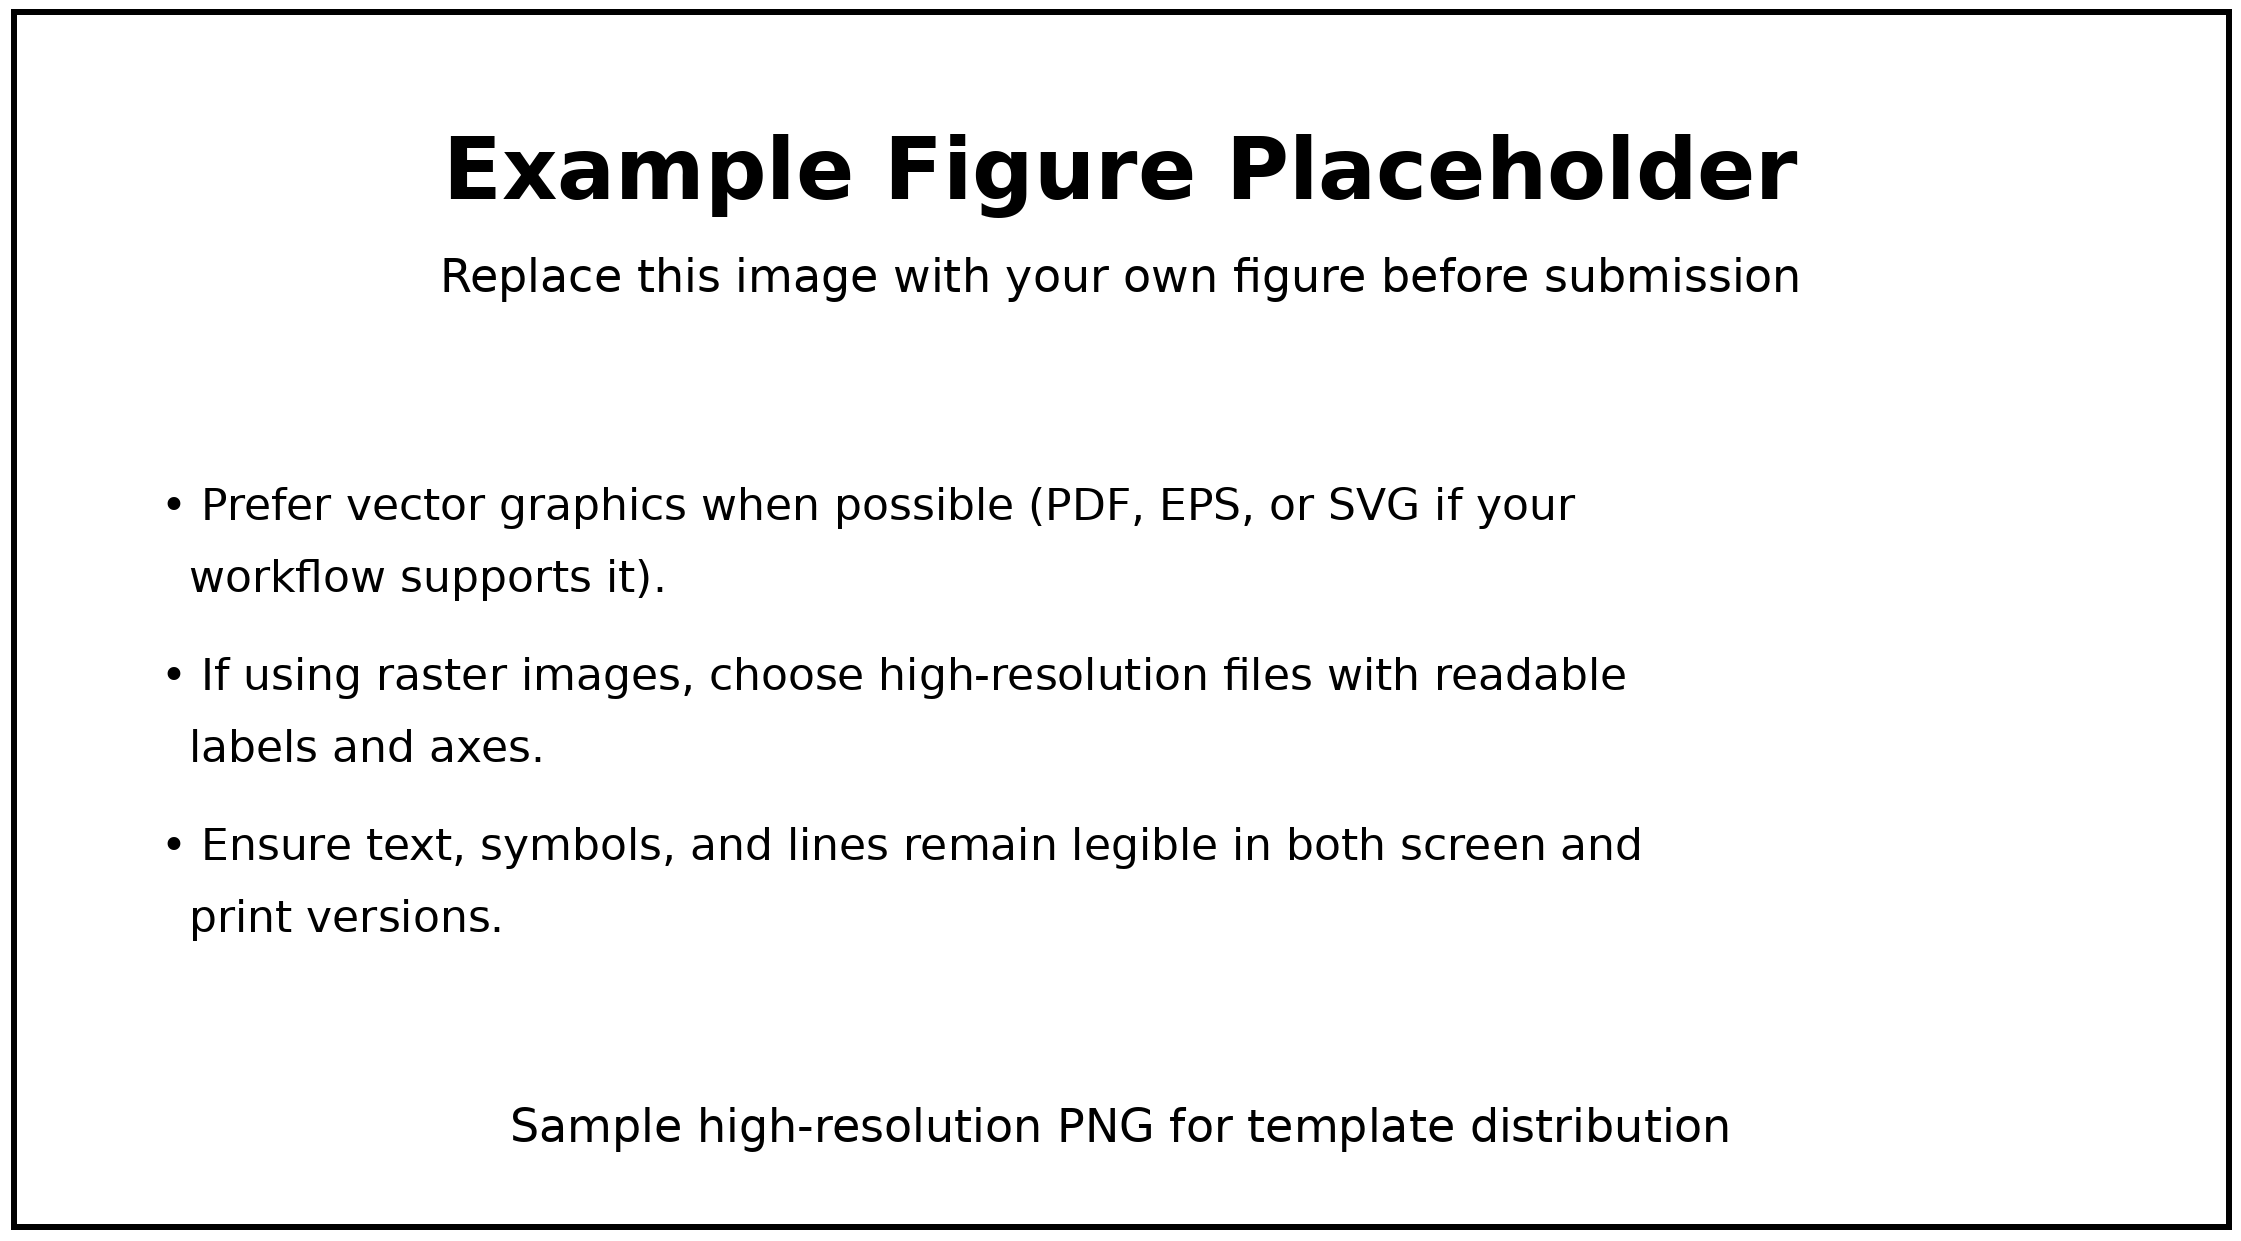
\includegraphics[width=0.9\columnwidth]{figs/example-figure.png}
\caption{Example of a figure caption.}
\label{fig_example}
\end{figure}

\subsection{Tables}
Tables should be numbered and cited in the text, as in Table~\ref{tab_example}. In IEEE style, captions are usually placed above the table. Authors are encouraged to keep table formatting simple, clear, and consistent throughout the manuscript.

\begin{table}[!b]
\caption{Example of a table caption}
\label{tab_example}
\centering
\begin{tabular}{cccc}
\hline
Item & Parameter & Factor & Value \\
\hline
A & Sample 1 & 1 & 123456 \\
B & Sample 2 & 2 & 567890 \\
C & Sample 3 & 7 & 142857 \\
\hline
\end{tabular}
\end{table}

\subsection{Equations}
Mathematical expressions should be centered and numbered consecutively when they are referenced in the text. For example, \eqref{eq_example} illustrates the format commonly used for displayed equations in technical papers. Similar mathematical notation is commonly found in signal processing, coding, and quality assessment literature \cite{ref:h264,ref:hevc,ref:ssim}.
\begin{equation}
E = mc^2
\label{eq_example}
\end{equation}

\subsection{Lists}
Bulleted or enumerated lists may be used when appropriate to improve clarity. For example, the main parts of a technical contribution may be summarized as follows:
\begin{itemize}
    \item presentation of the problem;
    \item description of the proposed approach; and
    \item discussion of the main results.
\end{itemize}

\lstinputlisting[
    style=python_style,
    linerange={11-},
    %firstnumber=11,
    caption={Calcular el área y perímetro de un círculo.},
    label={cod:punto1}
]{src/punto1.py}

\subsection{References}
References should be cited in the text using IEEE style, as illustrated by \cite{ref:kopka,ref:lamport}. All entries in the reference list should be complete, accurate, and consistently formatted according to the journal requirements. Examples of journal articles and technical references relevant to broadcast and media engineering are given in \cite{ref:h264,ref:hevc,ref:ssim,ref:setijbe}.

\section{Conclusion}
This demo paper has illustrated the basic structure and formatting expected for manuscripts submitted to the \textit{SET International Journal of Broadcast Engineering} (SET IJBE). The sample text has shown how to prepare typical elements of a submission, including the title, author information, abstract, keywords, sections, figures, tables, equations, lists, references, and acknowledgment section.

Authors are encouraged to replace all sample text with their actual material and to verify that the final manuscript complies with the requirements of SET IJBE.

\appendices
\section{Example of an Appendix}
Appendices may be used to provide supplementary material that is relevant to the paper but would interrupt the flow of the main text if included in the body of the manuscript. Typical examples include detailed derivations, additional tables, implementation notes, or complementary experimental results.

As an illustration, suppose that an intermediate result used in the main text is given by
\begin{equation}
y[n] = \sum_{k=0}^{M-1} h[k]x[n-k].
\label{eq_appendix_conv}
\end{equation}
Equation~\eqref{eq_appendix_conv} represents a discrete-time convolution and is included here only as a formatting example.

Authors should include appendices only when they add useful information for the reader. If no appendix is needed, this part of the template may simply be removed. If the paper is an Extended Abstract, appendices are not allowed.

% use section* for acknowledgment
\section*{Acknowledgment}
The authors would like to thank the supporting institutions and collaborators who contributed to this work.

% references section

\begin{thebibliography}{99}

\bibitem{ref:kopka}
H.~Kopka and P.~W. Daly, \emph{A Guide to \LaTeX}, 3rd~ed. Harlow, England: Addison-Wesley, 1999.

\bibitem{ref:lamport}
L.~Lamport, \emph{\LaTeX: A Document Preparation System}, 2nd~ed. Boston, MA, USA: Addison-Wesley, 1994.

\bibitem{ref:h264}
T.~Wiegand, G.~J. Sullivan, G.~Bjontegaard, and A.~Luthra,
  ``Overview of the H.264/AVC video coding standard,''
  \emph{IEEE Trans. Circuits Syst. Video Technol.}, vol.~13, no.~7,
  pp.~560--576, Jul.~2003, doi: \url{https://doi.org/10.1109/TCSVT.2003.815165}.

\bibitem{ref:hevc}
G.~J. Sullivan, J.-R. Ohm, W.-J. Han, and T.~Wiegand,
  ``Overview of the High Efficiency Video Coding (HEVC) standard,''
  \emph{IEEE Trans. Circuits Syst. Video Technol.}, vol.~22, no.~12,
  pp.~1649--1668, Dec.~2012, doi: \url{https://doi.org/10.1109/TCSVT.2012.2221191}.

\bibitem{ref:ssim}
Z.~Wang, A.~C. Bovik, H.~R. Sheikh, and E.~P. Simoncelli,
  ``Image quality assessment: From error visibility to structural
  similarity,'' \emph{IEEE Trans. Image Process.}, vol.~13, no.~4,
  pp.~600--612, Apr.~2004, doi: \url{https://doi.org/10.1109/TIP.2003.819861}.

\bibitem{ref:setijbe}
R.~N. Fonseca, M.~A. Ramirez, 
  ``Quality assessment of video in digital television,''
  \emph{SET Int. J. Broadcast Eng.}, 2015, doi: \url{https://doi.org/10.18580/setijbe.2015.1}.

\end{thebibliography}

% Author biographies should be omitted in Extended Abstract submissions.

\begin{IEEEbiography}[{
\includegraphics[width=1in,height=1.25in,clip,keepaspectratio]{figs/biophoto-one.png}}]{Author Number One} received the B.S. degree in electrical engineering from University Name, City, Country, in 2012, and the M.S. and Ph.D. degrees in communications engineering from University Name, City, Country, in 2015 and 2019, respectively.

Since 2020, Author Number One has been with the Department of Studies, Advanced Studies University, where they are currently an Associate Professor. Their research interests include broadcast systems, digital television, media transport, signal processing, and multimedia communications.

This author biography should be omitted in an Extended Abstract submission.
\end{IEEEbiography}

\begin{IEEEbiography}[{
\includegraphics[width=1in,height=1.25in,clip,keepaspectratio]{figs/biophoto-one.png}}]{Author N. Two} received the B.S. degree in electronics engineering from University Name, City, Country, in 2010, and the M.S. and Ph.D. degrees in electrical engineering from University Name, City, Country, in 2013 and 2018, respectively.

From 2014 to 2019, Author N. Two worked on research and development projects in digital communications and broadcasting systems. Since 2020, they have been with the Anonymous University, where they are currently a Professor. Their research interests include digital television, wireless systems, media delivery, coding technologies, and networked multimedia applications.

This author biography should be omitted in an Extended Abstract submission.
\end{IEEEbiography}

% insert where needed to balance the two columns on the last page with
% biographies
%\newpage

\begin{IEEEbiography}[{
\includegraphics[width=1in,height=1.25in,clip,keepaspectratio]{figs/biophoto-one.png}}]{Author N. Three} received the B.S. degree in computer engineering from University Name, City, Country, in 2011, and the M.S. degree in computer science from University Name, City, Country, in 2015.

Since 2016, Author N. Three has been with the Anonymous University, where they are currently a Researcher and Lecturer. Their professional and academic activities have focused on multimedia systems, interactive applications, audiovisual processing, and software platforms for digital media.

This author biography should be omitted in an Extended Abstract submission.
\end{IEEEbiography}

\end{document}
